\chapter{Machine Learning Background}
\label{chapter:background}

This chapter is intended to be a gentle introduction to the use of machine learning techniques and neural networks for supervised classification and regression. This is required for two reasons: most researchers are aware of neural networks, as it is a well known topic, but Convolutional Neural Networks are less covered in the teaching literature \footnote{For example, there is currently only one book for Deep Learning by Goodfellow et al. \cite{Goodfellow2016deep}}. The topic of Deep Learning is understood by many as just "more layers" in a network, without considering the recent advances in the field starting from 2012. Small contributions like the Rectified Linear Unit (ReLU) or the ADAM optimizer, or bigger ones like Dropout and Batch Normalization, have allowed to push the limits of neural networks.

We aim to fill the gap in that common knowledge, and to provide a self-contained thesis that can be read by specialists that do not know neural networks in detail. We also made the effort to cover in detail many practical issues when training neural networks, such as how to tune hyper-parameters, and the proper machine learning model iteration loop from the point of view of the neural network designer, as well as the best practices when using machine learning models.

We also summarize my experience training neural networks, as it is a process that contains equal parts of science and art. The artistic part is quite of a problem, as it introduces "researcher degrees of freedom" that could skew the results. One must always be aware of this.

Training a neural network is not an easy task, as it requires a minimum the following steps:

\begin{description}
	\item[Preprocessing] Training set must be carefully prepared. Input and output data must be normalized, typically to the $[0,1]$ or $[-1, 1]$ ranges, else the network might not converge.
	The initial training set must also be split into at least two sets: Training and Testing. Typically a third Validation set is also included in the split, in order to monitor network performance during training, and to detect overfitting.
	\item[Architectural Design] An appropriate network architecture has to be designed, or reused from previous designs. The learning capacity of a network must match or surpass the capacity required by the task to be learned. A big problem is that the task capacity is usually unknown and is difficult to estimate, which means network designers must use a trial-and-error approach. The learning capacity is related to the number of parameters (weights) in the network, but this relationship is not simple \footnote{A clear example is the general decreasing trend in the number of parameters in networks for ImageNet classification.}.
	\item[Training] The network must be trained using gradient descent with respect to a loss function. A key parameter controlling the convergence of this algorithm is the learning rate $\alpha$. If $\alpha$ is too big, then training might diverge \footnote{Divergence is signalled by a loss value going to infinity, or becoming NaN (Not a Number).}, while if $\alpha$ is too small, then convergence may be slow. The optimal value of the learning rate has to be found by experimentation on a validation set.
	\item[Testing] After the network has been trained and the loss indicates convergence, then the network must be tested. Many computational frameworks include the testing step explicitly during training, as it helps to debug issues. The testing step requires a validation set and metrics on this set are reported continuously during training.
	\item[Production Use] After many iterations of neural network development, once performance on various test sets is satisfactory, the network can be used in a production setting to perform predictions as needed.
\end{description}


It requires careful preparation of training data, then an appropriate network architecture has to be designed or reused from a previous design. 

\section{Classical Neural Networks}

The basic unit of a neural network is the neuron, which computes the function:
\marginnote{Activation Notation}

\begin{equation}
	\begin{split}
		z(\textbf{x}) &= \sum_i \textbf{w}_i \textbf{x}_i + b = \textbf{w} \cdot \textbf{x} + b  \\
		a(\textbf{x}) &= g(z(\textbf{x}))
		\label{background:neuron}	
	\end{split}
\end{equation}

Where $\textbf{x}$ is a input vector of $n$ elements, $\textbf{w}$ is a learned weight vector, and $b$ is a scalar bias that completes an affine transformation of the input. $g(x)$ is a scalar activation function, which is intended to introduce non-linear behavior into the network. A neural network with no activation function can just compute a linear combination of its input, and therefore is very limited on what tasks can be learned.

$a(\textbf{x})$ is called the activation\footnote{Do not confuse activation and activation function} of a neuron, while $z(\textbf{x})$ is usually called the pre-activation of a neuron, or just the output value before the activation is applied. This notation will be useful later.

\marginnote{Multilayer Perceptron} A neural network is then made by "stacking" a certain number of "layers", where each layer contains a predefined number of neurons. This is also called a Multilayer Perceptron (MLP). 
It is common to then represent inputs and outputs to each layer as vectors (or tensors), as this allows for explicit vector representation that can be easily accelerated in CPUs and GPUs. As an example, a three layer network would compute:

\begin{align*}
	z_1 &= \Theta_1 \cdot \textbf{x} + B_1\\
	a_1 &= g(z_1)\\
	z_2 &= \Theta_2 \cdot a_1 + B_2\\
	a_2 &= g(z_2)\\
	z_3 &= \Theta_3 \cdot a_2 + B_3\\
	a_3 &= g(z_3)
\end{align*}

Where now the $\Theta_i = \{ \textbf{w}_j \}_j$ is a matrix that contains the weights (row-wise) for the $i$-th layer, the input $\textbf{x}$ is a column vector and biases are stored in a row vector $\textbf{B}_i$. It should be noted that the number of neurons in each layer does not have to be the same, and the number of neurons in the last layer defines the output dimensionality of the network. Note than an alternate notation of $\Theta$ can include Biases $\textbf{B}$ as well, which is useful for a more direct implementation.

Training most machine learning models consists of minimizing a loss function $L$, which changes the model parameters in a way that the predictive performance of the model increases. In a sense, the loss function measures how well the model is doing with the current value of the parameter set. As neural networks usually have a large\footnote{AlexNet has 60 million trainable parameters (weights), ResNet has 20 million parameters, and VGG-16 has 138 million parameters.} number of parameters (the number of weights), unconstrained optimization algorithms are used to minimize the loss. The most common optimization algorithm is gradient descent.

Gradient descent uses the theoretical implications that the gradient of a scalar function points in the direction of maximum increase rate of that function. Then it is intuitive to think the rate of maximum decrease is exactly the opposite direction that of the gradient. Then gradient descent is an iterative algorithm that updates the parameters with the following relation:
\vspace*{1em}
\begin{equation}
	\Theta_{n+1} = \Theta_{n} - \alpha \nabla L(\hat{y}, y)
	\label{background:simpleGD}
\end{equation}

Where $\hat{y} = h_{\Theta_{n}}(\textbf{x})$ is the neural network output computed over inputs $\textbf{x}$ from a given dataset, with parameters $\Theta_n$, and loss function $L(\hat{y}, y)$. A key parameter in gradient descent is the \marginnote{Learning Rate} learning rate $\alpha$, which controls the "speed" at which the network learns. Intuitively the learning rate is a step size, as the gradient only provides a direction on which the parameters can be moved to decrease the loss, but not a magnitude on how much to move. This parameter has to be tuned in a validation set. If the learning rate is larger than necessary, then the loss value could oscillate or diverge. If the learning rate is too small, then convergence will be slow. The proper value of the learning rate will make convergence at an appropriate rate.

\subsection{Training as Optimization}

Training any machine learning model is typically formulated as an optimization problem. The most common formulation is the minimization of an objective function. This is typically called the \textit{loss function}, and it is designed in such a way that the model performance improves when the loss function decreases.

As previously mentioned, once a ML model is constructed, a loss function must be defined so the model can be trained. Gradient descent \marginnote{Gradient Descent} is the most common algorithm to train DNNs:
\vspace*{1em}
\begin{equation}
\Theta_{n+1} = \Theta_{n} - \alpha \nabla L(\hat{y}, y)
\label{background:fullGD}
\end{equation}

Where $\hat{y} = h_{\Theta_{n}}(\textbf{x})$ is the neural network output computed over inputs $\textbf{x}$ from a given dataset, with parameters $\Theta_n$, and loss function $L(h_{\Theta_{n}}(\textbf{x}), y)$. Gradient descent is an iterative algorithm and Eq \ref{background:fullGD} is executed for a predefined number of steps $n$. The value of the loss function at each step must be monitored as a simple check that the loss function is being minimized and is decreasing after each step.

The quality of the solutions obtained by gradient descent depends on several factors:

\begin{description}
	\item[Gradient Quality] Gradients must be of "high quality", which typically means that they must have many non-zero values. A related common problem is the vanishing gradient problem, specially in deeper networks, where the function composition nature of a DNN makes the gradients very small, slowing down or preventing training. Low quality gradients have many zero elements that prevent many parameters from converging to their optimal values.
	
	\item[Learning Rate] Setting the right value of the learning rate is a key factor to using gradient descent successfully. Typical values of the learning rate are $ \alpha \in [0, 1]$, and common starting values are $10^{-1}$ or $10^{-2}$.
	It is important that the learning rate is set to the right value before training, as a larger than necessary learning rate can make the optimization process fail (by overshooting the optimum or making the process unstable), a lower learning rate can converge slowly to the optimum, and the "right" learning rate will make the process converge at an appropriate speed.
	The learning rate can also be changed during training, and this is called  Learning Rate Schedule\marginnote{Learning Rate Schedule}. Common approaches are to decrease the learning rate by a factor after a certain number of iterations, or to decay the learning rate by a factor after each step.
	
	\item[Loss Surface] The geometry and smoothness of the loss surface is also key to good training, as it defines the quality of the gradients. The ideal loss function should be convex on the network parameters, but typically this is not the case for outputs produced by DNNs. Non-convexity leads to multiple local optima where gradient descent can become "stuck". In practice a non-convex loss function is not a big problem, and many theoretical results show that the local optima in deep neural networks are very similar and close in terms of loss value.
\end{description}

Gradient descent makes several implicit assumptions: the dataset fits into the computer's RAM, and that computing the loss function for the whole dataset is not an expensive operation. One forward pass of the complete network is required for each data point in the training set, and with complex neural networks and datasets of considerable size, these assumptions do not hold true.

\marginnote{Gradient Descent Variations} A simple way to overcome this problem is to only use part of the training set at a time during the training process. Assuming that the training set can be split into equal sized and non-intersecting sets, called batches, then we can iterate over batches, compute the loss function for a batch, compute the gradients, and apply one step of gradient descent. This is called Mini-Batch Gradient Descent (MGD):
\vspace*{1em}
\begin{equation}
\Theta_{n+1} = \Theta_{n} - \alpha \nabla L(h_{\Theta_{n}}(\textbf{x}_{i:j}), y)
\label{background:SGD}
\end{equation}

Where $\textbf{x}_{i:j}$ denotes that the neural network $h_{\Theta_{n}}(\textbf{x})$ and loss function $L$ are only evaluated for inputs $\textbf{x}_k$ where $k = [i, i + 1, i + 2, \dots, j]$. Then each batch is made by setting different values if $i$ and $j$, constrained to $i > j$ and $B = j - i$. The hyper-parameter $B$ is denoted the Batch Size \marginnote{Batch Size}. Typically batches are made by setting $B$ to a given value and using values $i, j = \{ (0, B), (B, 2B), (2B, 3B), \dots, (cB, n) \}$. Note that not all batches have the same size due that $B$ might not divide $|Tr|$ exactly. That means the last batch can be smaller. A variation of MGD is Stochastic Gradient Descent (SGD), where simply $B$ is set to one.
After approximately $\frac{|Tr|}{B}$ iterations of gradient descent, the learning process will have "seen" the whole dataset. This is called an Epoch \marginnote{Epochs}, and corresponds to one single pass over the complete dataset. Typically training length is controlled by another hyper-parameter, the Number of Epochs $M$.

Setting the value of the Batch Size $B$ is one hyper-parameter that controls the tradeoff between more RAM use during training, or more computation. It must be pointed out that MGD and SGD all introduce noise into the learning process, due to the approximation of the true gradient with the per-batch gradient. Larger values of $B$ use more RAM, but require less number of iterations, and additionally it reduces noise in the gradient approximation. Smaller values of $B$ require less RAM but more iterations and provide a more stable gradient approximation. It is common that $B$ is set such as the training process fills the maximum amount of RAM available\footnote{While training on a GPU, it is typical that the amount of GPU RAM is the only limitation to set $B$. The same applies while training on CPU but with system RAM.}.

The exact equations that compute gradients of the loss $\nabla L$ depend on network architecture. The back-propagation \cite[1em]{bishop2006pattern} algorithm is commonly referred to as a way to hierarchically compute gradients in multi-layer neural networks. In practice this algorithm is rarely used, as modern neural network frameworks such as TensorFlow and Theano use automatic differentiation \cite{baydin2017automatic} (AD) to compute gradients of the loss function automatically, making the developer's life much easier, as exotic architectures can be easily experimented.

\subsection{Loss Functions}

We now describe the most common loss functions used to train Neural Networks. A loss function is a scalar function $\mathbb{R}^n \times \mathbb{O} \rightarrow R^{+} \cup 0$ that gives a score to a set of predictions from a learning algorithm (typically a classifier or a regressor). Set $\mathbb{O}$ defines the ground truth labels, and in the case of regression it is typically $\mathbf{R}$, $[0, 1]$ or $[-1, 1]$. For classification then $\mathbb{O}$ is the set of classes, converted to a numerical form.

The most basic loss function is the mean squared error (MSE), typically used for regression:

\begin{equation}
	MSE(\hat{y}, y) = n^{-1} \sum_{i=0}^{n} (\hat{y}_i - y_i)^2
\end{equation}

The MSE loss penalizes the predicted values $\hat{y}$ that diverge from the ground truth values $y$. The error is defined just as the difference between $\hat{y}$ and $y$, and squaring is done to get a smooth positive value. One problem with the MSE is that due to the square term, large errors are penalized more heavily than smaller ones. This produces a practical problem where using the MSE loss might lead the convergence of the output to a mean of the ground truth values instead of predicting values close to them.
This issue could be reduced by using the Mean Absolute Error (MAE), which is just the mean of absolute values of errors:

\begin{equation}
    MAE(\hat{y}, y) = n^{-1} \sum_{i=0}^{n} |\hat{y}_i - y_i|
\end{equation}

The MSE is also called the $L_2$ loss, while the MAE is named as $L_1$ loss, both defined as the order of the norm applied to the errors. Note that the MAE/$L_1$ loss is not differentiable at the origin, but generally this is not a big issue. The $L_1$ loss can recover the median of the targets, in contrast to the mean recovered by the $L_2$ loss.

For classification, the cross-entropy loss function is preferred, as it produces a much smoother loss surface, and it does not have the outlier weighting problems of the MSE. Given a classifier that outputs a probability value $\hat{y}^c$ for each class $c$, then the categorical cross-entropy loss function is defined as:

\begin{equation}
	CE(\hat{y}, y) = -\sum_{i=0}^n \sum_{c=0}^C y_i^c \log \hat{y}_i^c
\end{equation}

Minimizing the cross-entropy between ground truth probability distribution and the predicted distribution is the equivalent to minimizing the Kullback-Leibler divergence \cite{mackay2003information}. For the case of binary classification, then there is a simplification usually called binary cross-entropy:

\begin{equation}
BCE(\hat{y}, y) = -\sum_{i=0}^n \left[ y_i  \log \hat{y}_i + (1 - y_i) \log (1 - \hat{y}_i) \right]
\end{equation}

In this case $\hat{y}$ is the probability of the positive class.

\subsection{Activation Functions}

There is a large selection of activation functions that can be used. A small summary is shown in Table \ref{background:activations}. The most common "classic" activation functions are the sigmoid and the hyperbolic tangent (TanH). These activation functions dominated the neural networks literature before 2010, as they produce the well known problem of vanishing gradient.

The vanishing gradient problem \marginnote{Vanishing Gradient Problem} happens when the gradient of the activation function becomes zero, and this is problematic because the network stops training. Looking at Figure \ref{background:saturatingActivations}, it can be seen that the activation function "saturates" when the input is small or large, making the gradient effectively zero. Stacking multiple layers that use sigmoid or TanH activation functions amplifies this effect and prevent the use of a large number of layers.

For this reason, sigmoid and TanH are called saturating activation functions \marginnote{Saturating Activation Functions}. This sparked the development of non-saturating activation functions, and the most well known of such functions is the Rectified Non-Linear Unit (ReLU) \cite{glorot2011deep}. The ReLu is a very simple function given by:

\begin{equation}
    g(x) = \max(0, x)
    \label{background:relu}
\end{equation}

This \marginnote{Rectified Linear Unit (ReLU)} activation function has constant output of zero for negative input, and a linear output for positive inputs. It should be noted that the ReLU is not differentiable at $x = 0$, as the slope at each side of the origin is different, but this usually poses no practical problem.

Use of the ReLU as activation function is one reason why Deep Learning is possible now. The breakthrough paper by Krizhevsky et al. \cite[-8em]{krizhevsky2012imagenet} mentions that using the ReLU as an activation function requires 4 times less iterations for GD to converge at the same loss value when compared to a sigmoid activation. There are multiple reports that using ReLU activations leads to loss surfaces that are easier to optimize and are less prone to local minima. One reason for this behavior is that the ReLU makes a network prefer sparse outputs.

\begin{table}[t]
	\centering
	\begin{tabular}{@{}lll@{}}
		\hline
		Name					& Range 			& Function\\
		\hline
		Linear					& $[-\infty, \infty]$	& $g(x) = x$\\
		Sigmoid					& $[0, 1]$			& $g(x) = (1 + e^{-x})^{-1}$\\
		Hyperbolic Tangent		& $[-1, 1]$			& $g(x) = (e^{2x} -1)(e^{-2x} + 1)^{-1}$\\
		\hline
		ReLU					& $[0, \infty]$		& $g(x) = \max(0, x)$\\
		SoftPlus				& $[0, \infty]$		& $g(x) = \ln(1 + e^x)$\\
		SoftMax					& $[0, 1]^n$		& $g(\textbf{x}) = (e^{x_i}) (\sum_k e^{x_k})^{-1}$\\
		\hline
	\end{tabular}
	\caption{Summary of commonly used activation functions.}
	\label{background:activations}
\end{table}

\begin{marginfigure}[-8em]
	\begin{tikzpicture}
	 	\begin{axis}[width = 0.9\textwidth, xlabel=, ylabel=Activation, ymin = -1.1, ymax = 1.1, legend style={at={(0.5, -0.3)},anchor=north}]
	 		\addplot+[mark=none] {1.0 / (1.0 + exp(-x))};
	 		\addlegendentry{Sigmoid}
	 		\addplot+[mark=none] {tanh(x)};
	 		\addlegendentry{TanH}

	 	\end{axis}
	 \end{tikzpicture}
	 \caption{Saturating Activation Functions}
	 \label{background:saturatingActivations}
\end{marginfigure}

Another commonly used activation function is the softmax \cite{bishop2006pattern}, and unlike the previously seen activations, it is not a scalar function. Instead the softmax takes a vector and transforms the input into a discrete probability distribution. This is very useful for multi-class classification, as a neural network can then output a probability distribution over class labels in $[0, 1, 2, \cdots, C]$. Then recovering the discrete class can be performed as taking the class with maximum probability. The vector definition of the softmax activation function is:

\begin{equation}
	g(\textbf{x}) = \left[ \frac{e^{x_i}}{\sum_j e^{x_j} } \right]_i
	\label{background:softmax}
\end{equation}

Given a softmax output $\textbf{a}$, the class decision can be obtained by:
\vspace*{1em}
\begin{equation}
	c = \argmax_i a_i
\end{equation}

\begin{marginfigure}
    \begin{tikzpicture}
    \begin{axis}[width = 0.9\textwidth, xlabel=, ylabel=Activation, ymin = -0.1, ymax = 4.0, xmin = -4.0, xmax = 4.0, legend style={at={(0.5, -0.3)},anchor=north}]
    \addplot+[mark=none] {max(0, x)};
    \addlegendentry{ReLU}
    \addplot+[mark=none] {ln(1 + exp(x))};
    \addlegendentry{Softplus}
    \end{axis}
    \end{tikzpicture}
    \caption{Non-Saturating Activation Functions}
    \label{background:nonSaturatingActivations}
\end{marginfigure}

Looking at Equation \ref{background:softmax} one can see that softmax outputs are then "tied" by the normalization value in the denominator. This produces a comparison operatiog between the inputs, and the biggest softmax output will always be located at the largest input relative to the other inputs. Inputs to a softmax  are typically called logits. As the softmax operation is differentiable, its use as an activation function then produces a loss surface that is easier to optimize.

Softmax combined with a categorical cross-entropy loss function is the base building block to construct DNN classifiers.

As the ReLU is not differentiable at $x = 0$ and it has constant zero output for negative inputs, this could produce a new kind of problem called "dying ReLU", where neurons that use ReLU can stop learning completely if they output negative values. As the activations and gradients become zero, the neuron can "get stuck" and not learn anymore. While this problem does not happen very often in practice, it can be prevented by using other kinds of activation functions like the Softplus function, which can be seen as a "softer" version of the ReLU that only has a zero gradient as the limit when $x \rightarrow -\infty$. Figure \ref{background:nonSaturatingActivations} shows the Softplus versus the ReLU activation functions. The Softplus function is given by:

\begin{equation}
	g(x) = \ln(1 + exp(x))
\end{equation}

Another similar activation function is the Exponential Linear Unit:
\vspace*{-0.1cm}
\begin{equation}
	g(x) = 
	\begin{cases}
		x       			& \quad \text{if } x \geq 0\\
		\gamma (e^x - 1) 	& \quad \text{if } x < 0\\
	\end{cases}
\end{equation}

There is a clear trend in recent literature about the use of learnable activations, where the activation function has a parameter that can be tuned during learning. Examples of this are the PReLU, Leaky ReLU and the MaxOut.

As a general rule, most deep neural networks use exclusively the ReLU as activation function, and when designing new networks, it should be preferred as it completely avoids the vanishing gradient problem.

\subsection{Weight Initialization}

SGD gives a way to iteratively improve the weight matrix to reduce some loss function that controls how and what the model is learning. But it does not specify the initial values of the weights. These are typically initialized by setting them to a random value drawn from some probability distribution. Weights cannot be initialized to zero, since this would lead to all neurons producing a zero value, and the network outputting constant zero, producing a failed learning process. Randomizing weights breaks the "symmetry" of initializing them to a particular value. If initial weights are too large, it could produce chaotic behavior (exploding gradients) and make the training process fail. There are many distributions that are used to draw initial weights:

\begin{description}
	\item[Uniform] Draw the weights from a Uniform distribution with a fixed range, parametrized by a scale parameter $s$. Popular values for $s$ are $s \in [0.1, 0.01, 0.05]$, and a common heuristic is to set $s = n^{-0.5}$, where $n$ is the dimensionality of the input to the layer.
        \vspace*{1em}
		\begin{equation}
			w \sim U(-s, s)
		\end{equation}
	\item[Gaussian] Draw the weights from a Gaussian distribution with a fixed standard deviation. Popular values are $\sigma \in [0.1, 0.01, 0.05]$
        \vspace*{1em}
		\begin{equation}
			w \sim N(0, \sigma)
		\end{equation}
	\item[Glorot or Xavier] Named after Xavier Glorot \cite{glorot2010understanding}. Draw the weights from:
		\begin{equation}
			w \sim U(-s, s) \qquad s^2 = \frac{6}{F_{in} + F_{out}}
		\end{equation}
         Where $F_{in}$ is the number of input elements to the neuron, and $F_{out}$ is the number of output elements. This initialization scheme is based on the intuition that variance of the input and output should be approximately equal for a stable behavior at the beginning of training, which implies that initial weights are scaled differently depending on the dimensionality of the inputs and outputs.
	\item[Orthogonal] Draw weights from a random orthogonal matrix, after applying gain scaling \cite[-6em]{saxe2013exact}. This method is theoretically grounded and guarantees that convergence will be achieved in a number of iterations that is independent of network depth. The weight matrix is generated by first generating a random matrix with elements $w_{ij} \sim N(0, 1)$, then performing Singular Value Decomposition on $w$, and then picking either the $U$ or $V$ matrices depending on the required output dimensionality. Finally this matrix is scaled by a gain factor $g$ that depends on the activation function, in order to ensure stable learning dynamics.
\end{description}

Biases $b$ can also be initialized with the same scheme as weights, but there is no problem if bias are initialized to zero, and some authors prefer this. We have shown a small subset of weight initialization schemes available in the literature, and overall there is no consensus if one is superior to another, and in general it does not matter much which one is chosen, as other learning tools\footnote{Like Batch Normalization, Dropout, and Non-Saturating Activation Functions.} can be used to provide superior training stability. Before these techniques were known, the neural network designed had to carefully adjust the weight initialization scheme in order for learning to converge to a useful solution.

\subsection{Data Normalization}

One key technique that always must be used \footnote{My experience from answering Stack Overflow questions is that too many people do not normalize their data, making training their networks much more difficult.} is data normalization. As the input and output data typically comes from real sources, it is contaminated by non-ideal behaviors, like different scales for each feature, or simply are in a range that typical neural networks have issues modeling.

The scale of input features is an important issue as if inputs have different ranges, then the weights associated to those features will be in different scales. Since we usually use fixed learning rates, this leads to the problem that some parts of a neuron learn at different speeds than others, and this issue propagates through the network, making learning harder as the network becomes deeper.

The scale of outputs poses a different but easier problem. The designer has to make sure that the range of the activation of the output layer matches the range of the desired targets. If these do not match, then learning will be poor or not possible. Matching the ranges will make sure that learning happens smoothly.

\begin{description}
	\item[Min-Max Normalization] Normalize each component of the input vector by subtracting the minimum value of that component, and divide by the range. This produces values in the $[0, 1]$ range.
    
		\begin{equation}
			\hat{x} = \frac{x - \min_i x_i}{\max_i x_i - \min_i x_i}
		\end{equation}
		
	\item[Z-Score Normalization] Subtract the sample mean $\mu_x$ and divide by the sample standard deviation $\sigma_x$. This produces values that are approximately in the $[-1, 1]$ range.
    
		\begin{equation}
			\hat{x} = \frac{x - \mu_x}{\sigma_x}
		\end{equation}
        \begin{equation}
            \mu_x = n^{-1} \sum x_i \qquad \sigma_x = \sqrt{(n-1)^{-1} \sum (x_i - \mu_x)^2}
        \end{equation}
        
    \item[Mean Substraction] Typically used to train models that take images as inputs \cite{krizhevsky2012imagenet}. Images are represented either as tensors $(W, H, C)$ with values in the $[0, 255]$ or $[0, 1]$ range, and they are normalized by computing the mean image over the training set, or the individual per-channel means over the training set, and subtracting this mean from each image, which overall will produce values in the $[-128, 128]$ or $[-0.5, 0.5]$ range.
\end{description}

\subsection{Regularization}

Regularization is a way to control the learning capacity of a machine learning model, by imposing constraints or prior information to bias the model to a preferred configuration. There are many ways to regularize neural networks, and in this section we will describe two modern regularization techniques: Dropout and Batch Normalization.

A common view of regularization from statistical learning theory is that it controls the number of trainable parameters, which is related to overfitting \cite[-5em]{bishop2006pattern}, but a more recent view \cite[-2em]{luo2018understanding} is that the number of parameters does not completely explain overfitting and the expected predictive performance at inference time.

Dropout \marginnote{Dropout} is a technique pioneered by Srivastava et al \cite[1em]{srivastava2014dropout}. The authors of Dropout noticed that when a neural network overfits, the neurons inside it \textit{co-adapt} or their outputs become correlated. This reduces model efficiency and generalization greatly. They proposed that this co-adaptation can be broken by introducing noise in the activations, and they choose a model that produces a mask $\mathbf{m}$ of length $n$ where each element is Bernoulli distributed with probability $p$: $m_i \sim \text{Bernoulli}(p)$.

Then this mask is multiplied with the activations of a particular layer, which has the effect of \textit{turning off} some activations of a layer, and letting others pass unchanged. This is called the dropout mechanism. During training the masks at each Dropout layer are randomly sampled at each iteration, meaning that these masks change during training and mask different activations at an output. This breaks any correlations between activations in one layer and the one before it (where the Dropout layer is placed), meaning that more strong features can be learned and co-adaptation of neurons is prevented.

At inference or test time, Dropout layers do not perform any stochastic dropping of neurons, and instead they just multiply any incoming activation by $p$, which accounts for all activations being present during inference, unlike at training time. This also prevents any kind of stochastic effect during inference. It should also be noted that Dropout can also be used with its stochastic behavior at inference time, which produces very powerful model uncertainty estimates, as it was proven by Gal et al 2015. \cite{gal2015dropout}.

Using Dropout layers in a neural network, typically before fully connected ones, has the effect of reducing overfitting and improving generalization significantly.

Dropout can also be seen as a way of Bayesian model averaging \cite{gal2016uncertainty} as when dropping neurons at training time, new architectures with less neurons are produced, which are then averaged at inference time, which is a theoretical explanation of why Dropout works and improves generalization. Note that while the number of effective parameters during training is reduced by Dropout (by a factor of $p$) due to the dropping of activations, during inference/testing the number of parameters does not change, and all parameters are used to make a prediction.

Another technique that can be used for regularization is Batch Normalization \cite[1em]{ioffe2015batch}. This technique was not specifically designed to reduce overfitting in neural networks, but to increase convergence speed while training. The authors of Batch Normalization also noticed that it has a powerful regularization effect, and most current deep neural networks are trained with it, as it improves generalization almost "for free".

Batch Normalization \marginnote{Batch Normalization} is based on the concept of internal covariate shift reduction. Given a set of layers, the covariate is the empirical probability distribution of their outputs. Covariate shift is the change of that distribution as training progresses. Internal covariate shift is the covariate shift of the hidden layers of a neural network. The intuition for Batch Normalization is that drastic internal covariate shift is prejudicial for neural network training, as it is more likely to saturate non-linearities, and unstable activation distributions will need more training iterations to converge successfully. Both situations causes slow training convergence.

Reducing the internal covariate shift can be achieved by normalizing the activations (before applying a non-linearity). As typical decorrelation methods like PCA or ZCA whitening are too expensive to use during neural network training (specially with high dimensional data), the Batch Normalization authors proposed two simplifications.

The first is to perform Component-Wise Normalization along the features. Given a vector of activations $\textbf{x}$, as a middle step for layer output computation, then each component of that vector should be normalized independently, by using a simple mean and standard deviation normalization: 
\vspace*{1em}
\begin{equation}
    \mu_{B} = |B|^{-1} \sum x_i \qquad \sigma^2_{B} = |B|^{-1} \sum (x_i - \bar{x})
\end{equation}

The normalization happens along the features dimension of the a mini-batch of activations. This allow for an efficient implementation using SGD. Normalizing a mini-batch $\textbf{x} \in B$ of size $|B|$ is performed as:
\vspace*{1em}
\begin{equation}
    \hat{x}_i = \frac{x_i - \mu_{B}}{\sqrt{\sigma^2_{B} + \epsilon}}
\end{equation}

Where $\epsilon = 0.001$ is a small constant to prevent division by zero. Normalizing activations has the unintended effect of destroying the representation capability of the network, but it can be easily restored with a linear transformation:
\vspace*{1em}
\begin{equation}
    y_i = \gamma_i \hat{x}_i + \beta_i
\end{equation}

Where $\gamma_i$ and $\beta_i$ are scalar parameters that are learned using gradient descent\footnote{These parameters are added to the set of learnable parameters in a layer}. It should be noted that this transformation does not correspond to a fully connected layer, as these are per-feature scaling and bias coefficients for the activation instead.

At inference time, mini-batch statistics are not available, as many inference calls use a single test sample. Fixed normalization coefficients can then be estimated from the training set and used during inference. This is performed as part of the learning process as a exponentially averaged running mean and variance of the mini-batch activation statistics, but with an unbiased variance estimate $\frac{n}{n-1} E[\sigma^2_{B}]$ used instead.

Recently more advanced versions of activation normalization schemes have appeared in the literature, such as Layer Normalization \cite[-7em]{ba2016layer}, Instance Normalization, and Group Normalization \cite[-2em]{wu2018group}. These methods expand Batch Normalization to specific use cases and make it less dependent on mini-batch sizes.

The inclusion of Batch Normalization in neural network architectures is considered to be a good practice, and most modern neural network architectures (like ResNet, GoogleNet, DenseNets, etc) use it. Using batch normalization has a regularizing effect, generally improving performance. There is strong evidence that this is due to a smoother loss surface \cite[-6em]{santurkar2018does} as the result of activation normalization, and not to a reduction in the covariate shift, as the original paper argues.

Luo et al. \cite{luo2018understanding} provide a theoretical framework for the understanding of the regularization effect of Batch Normalization. They find that Batch Normalization is an implicit regularized that can be decomposed into population normalization and gamma decay, the latter being an explicit regularizer. These results show that Batch Normalization of CNNs shares many properties of regularization.

Classical regularization techniques for machine learning models can also be used for neural networks, and the most common ones are $L_1$ and $L_2$ regularization \marginnote{$L_1$ and $L_2$ Regularization or Weight Decay} (also called Weight Decay). Both of them add a term $\lambda \sum_i ||w_i||^p$ to the loss function, which penalizes large weights that are not supported by evidence from the data. $p$ is the order of the norm that is being computed over the weights.

\subsection{Optimizers}

Optimizers are algorithms that perform minimization of the loss function through gradient descent, as mentioned previously. The standard formulation of SGD uses a constant learning rate, but in practice this does not have to be the case, and a rich literature\cite{ruder2016overview} exists on optimization methods that scale the learning rate with gradient information, so an individual learning rate is used for each trainable parameter in $\Theta$.

The most straightforward way to incorporate this idea is to use the square root of the sum of past squared gradients as a scaling factor for the learning rate. An optimizer using this idea is AdaGrad \cite{duchi2011adaptive}, with the update rule:
\vspace*{1em}
\begin{align}
    g_n &= \nabla L(h_{\Theta_{n}}(\textbf{x}_{i:j}), y)\nonumber \\
    r_n &= r_{n-1} + g_n \odot g_n\nonumber\\
    \Theta_{n+1} &= \Theta_{n} - \alpha \frac{g_n}{\epsilon + \sqrt{r_n}}
    \label{background:AdaGrad}
\end{align}

Where $\odot$ represents component-wise multiplication, and $\epsilon$ is a small constant for numerical stability and to prevent division by zero. The gradient is divided scaled component-wise by the square root of sum of gradients as well, in order to scale the learning rate for each parameter independently. AdaGrad works most of the time, but the use of a complete history of gradients makes it unstable, since any gradient disturbance at the beginning of training would over-reduce the gradients and prevent the model from reaching its full potential.

An alternative to AdaGrad is RMSProp \cite{tieleman2012lecture}, where instead of keeping a sum of the full history of squared gradients, a moving exponential weighted average is kept, so older squared gradient are given less importance than more recent ones. The update rule is:
\vspace*{1em}
\begin{align}
    r_n &= \rho r_{n-1} + (1 - \rho) g_n \odot g_n\nonumber\\
    \Theta_{n+1} &= \Theta_{n} - \alpha \frac{g_n}{\sqrt{\epsilon + r_n}}
    \label{background:RMSProp}
\end{align}

Where $\rho$ is a decay parameter that controls the weight of past squared gradients through the moving average, usually it is set to $0.9$ or $0.99$. RMSProp is more stable than AdaGrad due to better control of the history of squared gradients, and allows a model to reach a better optima, which improves generalization. It is regularly used by practitioners as one of the first methods to start training a model.

Another advanced Optimizer algorithm is Adam \cite[-1cm]{kingma2014adam}, which stands for \textit{adaptive moments}. Adam combines improvements of RMSProp with direct application of momentum in the gradient update. The authors of Adam found that the exponentially weighted averages are biased, and correct this bias using a term that depends on the decay parameter of the exponential weight averages. Additionally, Adam applies an exponential weighted average to the gradient itself, which is equivalent to performing momentum on the gradient update. The update rule is:
\vspace*{1em}
\begin{align}
    s_n &= \rho_1 s_{n-1} + (1 - \rho_1) g_n\nonumber\\
    r_n &= \rho_2 r_{n-1} + (1 - \rho_2) g_n \odot g_n\nonumber\\
    \Theta_{n+1} &= \Theta_{n} - \alpha \frac{s_n}{\epsilon + \sqrt{r_n}} \frac{1 - \rho_2^n}{1 - \rho_1^n}
    \label{background:Adam}
\end{align}

Where $s_n$ is the biased estimate of the gradient and $r_n$ is the biased estimate of the squared gradients, both obtained with an exponential moving average with different decay rates $\rho_1$ and $\rho_2$. The factors $1 - \rho_1^n$ and $1 - \rho_2^n$ are used to correct bias in the exponential moving averages. These computations are done component-wise.

Overall Adam performs considerably better than RMSProp and AdaGrad, training models that converge faster and sometimes obtain slightly better predictive performance, but this is not always the case. Recent advances have shown that Adam can be improved as there are some theoretical issues \cite{reddi2018convergence} that have been fixed.
Adam is generally preferred by practitioners when training a newly designed model, as it requires less tuning of the learning rate.

The use of advanced Optimizer algorithms makes tuning the learning rate an easier task, and in some cases it allows the use of larger learning rates, which translates into faster convergence and lower training times. The only disadvantage of using Optimizers is that sometimes the learning process does not converge to the \textit{best} optimum\footnote{For example, it is well known in the community that using Adam on a VGG-like network fails to converge, and we have experimentally confirmed this, the loss just does not decrease, plain SGD works perfectly.}, and there are increased memory usage to store the exponentially weighted averages, usually by $100 \%$ for RMSProp and AdaGrad, and by $200 \%$ for Adam, which can constraint the kind of models that can be trained on a GPU.

\subsection{Performance Evaluation}

The idea of using machine learning models is to learn to generalize, that is, learn a model from a limited set of data that is useful for samples that the model has never seen during training. A useless model only performs well in the training set.

An \marginnote{Cross Validation} important part of designing a machine learning model is related to its desired performance. This is measured by the loss function during training, but just minimizing it in the training set does not guarantee any kind of performance in new and unseen samples. For this an additional set is needed, called the test set. A model is trained on the training set, and its performance evaluated on the test set, which provides an unbiased estimate of the generalization performance of the model. This is typically called Cross Validation.

Typically \marginnote{Train, Validation, and Test Splits} the available data is randomly split into three datasets: the Training set, the Validation set, and the Test set. The fractions for each split vary, but it is ideal to make the biggest split for the training set, at least 50 \% of the available data, and use the rest in equal splits for the validation and test sets.

The validation set is used to evaluate performance during hyper-parameter selection, and only after fixing these values, a final evaluation on the test set can be performed. This prevents any kind of bias in samples in the training or validation set from affecting conclusions about model performance.

Overfitting \marginnote{Overfitting} is the problem where the model learns unwanted patterns and/or noise from the training data, and fails to generalize outside of its training set. Detecting overfitting is key during training any machine learning model, and is the reason why validation or test sets are used, as it is the only known way to detect overfitting.

During the training process, the loss and metrics on the training set is typically tracked and displayed to the designer, and after each epoch, loss and associated metrics can be computed on the validation set. The overall pattern of both training and validation loss tells a picture about that is happening, we cover three cases:

\begin{description}
    \item[Training Loss Decreasing, Validation Loss Decreasing] Indicates that the model is learning and also generalizing well. This is the ideal case.
    \item[Training Loss Decreasing, Validation Loss Increasing] Indicates that the model is overfitting, as more noise is learned from the training set, which does not generalize to the validation set.
    \item[Training Loss Not Decreasing, Validation Loss Not Decreasing] The model is not overfitting, but it indicates that the model does not fit the data. A model with more learning capacity might be needed, as the current model cannot really predict the data given the input features. For example, if fitting a linear model to data with a quadratic shape. This case might also indicate that the input features might not be well correlated to the desired output or that the learning problem is ill-defined.
\end{description}

For classification problems, the loss is typically the cross-entropy and its variations, but humans prefer to evaluate performance with the accuracy \marginnote{Accuracy} metric, as it is directly interpretable:
\vspace*{1em}
\begin{equation}
    \text{ACC}(\hat{y}, y) = n^{-1} \sum \mathbb{1}[y = \hat{y}]
\end{equation}

Accuracy is just the fraction of samples that are correctly classified, that is, the predicted label $\hat{y}$ is the same as the ground truth label $y$. Note that the accuracy metric is completely meaningless for regression problems, as a continuous output equality is ill-defined. One way to define accuracy for continuous outputs is to consider equality if prediction differs from ground truth by not more than a given $\epsilon$, or to use pearson's correlation coefficient $R$, or the $R^2$ coefficient of determination.

\subsection{Hyper-parameter Tuning}

Hyper-parameters are all parameters in a model that need to be decided before starting the learning process, and that cannot be directly learned (as in by a learning algorithm) from data. The values of these parameters must be decided by the human designer. This also includes the neural network architecture.

A general way to tune these parameters is to use Grid Search \marginnote{Grid Search}. For this process, a range of values is defined for each parameter $P_i$, and each range is discretized to a finite set of values that will be tested. Then a grid is built by all possible combinations of parameter values $S = P_0 \times P_1 \times P_2 \times \cdots \times P_n$. For each value in the parameter space $S$, a model is trained and evaluated on the validation set. The set of parameters that produces the lowest validation loss is used to build the full model, but this is not the only possible criteria.
It is common that many sets of parameters provide the same or similar performance than the best model, so other criteria could be used, such as minimizing the number of total weights in the model, or maximizing computational performance subject to a given learning performance.

Grid Search is computationally expensive, as making the grid will exponentially explode the number of parameter sets that have to be tried, and training a neural network for each of these parameter sets is also computationally expensive. A common observation after performing grid search is that some parameters are not really important, having only a small or zero effect on learning performance.

For\marginnote[-2em]{Random Search} this reason, Random Search \cite{bergstra2012random} was proposed, where instead of using discrete values for the parameters, probability distributions are used to model each parameter, and during the search process, a parameter set is drawn by sampling each parameter distribution, and a model trained and evaluated.
Random Search has the advantage of minimizing the use of computational budget on uninteresting parameters, and it has been experimentally proven to obtain the same or slightly better models than Grid Search, with less computational budget. Note that since the exploration of the parameter space is random, the bias from parameter values set by the designer can potentially be reduced, and even work in other datasets for which random search is being performed.

Two parameters deserve special consideration due to their effect on the learning process: the learning rate (LR) and the number of training epochs.

\begin{description}
    \item[Learning Rate] This parameter controls the "speed" over which learning is performed, as it scales the gradient, which effectively makes it a kind of step size in the parameter space. Valid learning rate values are typically in the $[0, 1]$ range, but small values are mostly used in practice. If a large LR is used, then learning could diverge (producing infinite or NaN loss values), if a too small LR is used, learning happens but very slowly, taking a large number of epochs to converge. The \textit{right} LR value will produce fast learning, with a loss curve that is similar to exponential decay. Figure \ref{background:effectLR} shows typical loss curves with different learning rates. The case of a high LR shows that in the case where learning does not fail, but the loss decreases and stays approximately constant after a certain number of epochs. Note that the LR does not have to be a constant, and it can be varied during training. The typical method is to decrease the LR by a factor after a \textit{plateau} of the loss curve has been detected, which potentially could allow the loss to decrease further.
    
    \begin{marginfigure}
        \begin{tikzpicture}
            \begin{axis}[width = \textwidth, xlabel={Epochs}, ylabel={Loss},
            xmin = 0.0, xmax = 100.0, ymin = 0.0, ymax = 10.0,
            legend style={at={(0.5, 2.0)},anchor=north}]
                \addplot+[mark=none, domain=0:100] {10 - 0.09 * x + 0.5 * rnd};
                \addlegendentry{Low LR}
                \addplot+[mark=none, domain=0:100] {exp(2.5 - 0.1 * x) + 0.4 * rnd};
                \addlegendentry{Correct LR}
                \addplot+[mark=none, domain=0:100] {exp(2.0 - 0.05 * x) + 2 + 0.6 * rnd};
                \addlegendentry{High LR}
            \end{axis}
        \end{tikzpicture}
        \caption{Effect of Learning Rate on the Loss Curve during Training}
        \label{background:effectLR}
    \end{marginfigure}
    
    Learning rate can be tuned using grid or random search, but a faster way is to guess an initial LR, train different models and vary the learning rate manually, decreasing or increasing it accordingly to the previously mentioned rules. A common heuristic \cite{Goodfellow2016deep} is that if learning fails, decrease the LR by a factor of ten until the loss starts to decrease consistently, and adjust further by small steps to produce the ideal loss curve. Typical learning rates used in the literature are negative power of 10, like $\alpha = [0.1, 0.01, 0.001]$.
    
    \item[Number of Epochs] This parameter controls the length of the training process. If a model is trained for a short number of epochs, then it might not have converged, meaning that the loss could have continued to decrease if trained for longer, while training for more epochs than necessary risks overfitting, assuming no regularization was used.
    
    The number of training epochs can be tuned by experimenting manually in a similar way as the learning rate. The designer could set an initial number of epochs (say, 10) and then increase or decrease it accordingly if the loss shows no signs of convergence \footnote{A model has converged when the training process shows that the loss function can no longer decrease, and the loss shows a wiggling behavior, staying approximately constant.}, or if the model overfits.
    
    Related to this parameter is the early stopping criterion, \marginnote[0.5cm]{Early Stopping} where validation loss is monitored after each epoch, and training stopped if the validation loss starts to increase consistently after a tunable number of epochs. This prevents overfitting and would only require to tune a reasonable minimum number of epochs. The designer should also make sure to tune the learning rate appropriately, as the constant loss that indicates convergence could also be caused by a learning rate that is too high.
\end{description}

Note that both the value of learning rate and number of epochs depend on the actual loss function that is being minimized, any change to the loss implies retuning both parameters, as the actual loss surface or landscape is what defines the learning rate and length of training.

\section{Convolutional Neural Networks}

Convolutional Neural Networks (usually abbreviated CNNs or ConvNets) were introduced by Yann LeCun \cite{lecun1998gradient} in the 90's, initially for the task of handwritten object recognition, but they have been successfully applied to other vision tasks, like Object Detection and Localization, Semantic and Instance Segmentation, and Image Super-Resolution, etc. CNNs have revolutionized computer vision, as now many visual tasks can be learned using neural networks that are specifically designed for image processing.

This kind of networks are designed to process images as inputs and they have an optimized network structure to exploit three common properties of images:

\begin{description}
	\item[Local Statistics] In images the correlation between neighboring pixels in a region is higher than the correlation of far away pixels. This observation also has a biological counterpart as the receptive field in the visual cortex, where cells are excited by patterns in regions of the visual field.
	
	This property is implemented by a CNN by using neurons that are connected to a neighboring region in the input image. This is represented by a convolution filter or kernel, which can be square or rectangular. After convolution of the input image with a certain number of filters (one for each neuron), such layer produces the same number of output images called feature maps.
	
	\item[Translation Invariance] Generally the filters in that \textit{look} into a neighboring region of the input image do not depend on a spatial position in the image. Filters are generic and should be useful in any part of the image. This is one kind of translation invariance, since instead of connecting a neuron with all pixels of the input image, which increases the number of parameters, we can only learn the weights associated to the filter, and run it over the whole input image in a sliding window manner, which is effectively the convolution operation.
	
	Another kind of translation invariance is downsampling. When the network \textit{looks} for relevant features to detect or recognize objects, the convolution filter might produce high responses at several neighboring positions. One way to filter these high responses is to perform pooling on a feature map, which will only keep the high responses and discard irrelevant information, as well as reducing the dimensions of a feature map.
	This allows the network to concentrate on important features, and since pooling is invariant to small translations (inside the pooling region), this introduces a small degree of translation invariance into the network design.
	
	\item[Feature Extraction] In most computer vision tasks, features are used to discriminate relevant parts of an image. These features are manually engineered by researchers, which is a labor intensive task. Instead, a CNN can learn relevant features to the problem by means of learning the weights of convolution filters.
	This is a very important property of CNNs, features can automatically be learned directly from the training data, since the feature extraction and classifier modules are both part of the same neural network, which can be trained end-to-end. This means that relevant features for each vision problem can be learned directly from the data, without any manual engineering and with minimal preprocessing \footnote{In general this preprocessing consists of dataset augmentation and input/output normalization.}.
\end{description}

The basic design of CNNs introduces two new types of layers: Convolution and Pooling layers.

Images are usually represented as multi-dimensional arrays or tensors, \marginnote{Image Representation} with shapes $(W, H, C)$, where $W$ is the width, $H$ is the height, and $C$ is the channels dimension, \footnote{This is also referred as depth dimension in some papers.} which is one for a grayscale image, and three for a RGB color image. This representation also allows for arbitrary numbers of channels, and it will be useful later on.

\subsection{Convolutional Layers}

For a convolutional layer \marginnote{Convolutional Layer}, the output $y$ is given by:
\vspace*{1em}
\begin{equation}
    y = f(\mathbf{x} \ast \mathbf{F} + b)
\end{equation}

Where $\ast$ is the convolution operation, $x$ is the input image, $\mathbf{F}$ is the convolution filter (weights), $b$ is a bias and $f$ is a non-linear activation function that is applied element-wise to the output. In other words, a convolution layer takes an image as input, convolves it with a filter, adds a bias, and then passes the convolved image through a non-linear activation function. The output of a this kind of layer is called a \textit{convolutional feature map} \marginnote{Convolutional Feature Map}, as it represents visual features of an image (a map).

In practice, convolutional layers use more than one filter per layer, as this allows to learn different kinds of features at the same time, and later it allows the learning of feature hierarchies \cite{zeiler2014visualizing}. This is represented as a layer taking inputs of shape $(W, H, C)$, and the output having shape $(W, H, K)$, where $K$ is the number of filters in the convolution layer. Each filter is convolved individually with the input image, and the result after applying bias and activation function is stored in the channels dimension of the output, stacking all feature maps into a 3D volume. Convolutional layers can also take feature maps as inputs, which forms the feature hierarchy previously mentioned.

Another important detail of a convolutional layer is that both bias and weights on the filter are learned using gradient descent. They are not hand tuned as previously was done for image processing, like to make edge detection or sharpness filters. The filter in a convolutional layer is not necessarily a two dimensional matrix, as when the input image or feature map has $K > 1$ channels, then the filter must have a matching shape $(W, H, K)$, so convolution can be possible. When the filter has multiple channels, convolution is performed individually for each channel using the classical convolution operation from image processing \cite[-1em]{gonzalezDIP2006}.

The filter size (width and height) in a convolutional layer is a hyper-parameter that must be tuned for specific applications, and generally it must be a odd integer, typical values are $3 \times 3$ or $5 \times 5$, but some networks such as AlexNet \cite{krizhevsky2012imagenet} used filter sizes up to $11 \times 11$. The width and height of a filter do not have to be the same, but generally square filters are used.

Convolution is normally performed with a stride of 1 pixel \marginnote[1em]{Stride}, meaning that the convolution sliding window is moved by one pixel at a time, but different strides can also be used which is a kind of sub-sampling of the feature map.

The output dimensions of a convolutional layer are defined by the filter sizes, as convolution is only typically performed for pixels that lie inside the image region, and out of bound pixels are not considered (at the edges of the image). Padding \marginnote{Padding} can be added to the input image or feature map in order to output the same spatial dimensions as the input.

For a $N \times N$ filter and a $W \times W$ input image or feature map, with padding of $P$ pixels and stride $S$, the output has dimensions $O$:
\vspace*{1em}
\begin{equation}
    O = \frac{W - N + 2P}{S} + 1
\end{equation}

\subsection{Pooling Layers}

A pooling layer is used to introduce a small degree of translation invariance to the network design, and to control the flow of information through the network, by performing down-sampling on feature maps. This works by forcing the network during learning to produce meaningful features that will pass through the pooling operation. 

Pooling works by partitioning \marginnote{Down-sampling} an input feature map of size $W \times H$ in non-overlapping regions of the same size $D \times D$, and then performing a aggregation operation on each region, producing a scalar value, and then replacing each region with this aggregated scalar value, effectively performing down-sampling, as the output of the pooling operation has size $\frac{W}{D} \times \frac{H}{D}$. $W$ and $H$ must be divisible by $D$ or else padding is required. Pooling can be performed in overlapping regions, as well as with a stride $S > 1$, depending on the designer's needs.

Two types of aggregation operations are used in the CNN literature:

\begin{description}
    \item[Max-Pooling] The maximum value in each region $R$ is kept and used as output:
        \vspace*{1em}
        \begin{equation}
            y = \max_{x \in R} x 
        \end{equation}
        
        The concept of Max-Pooling is that only the maximum activation in each region of the feature map will pass, suppressing the non-maximums. While it works well in practice, there are issues since small disturbances to the activations in a feature map will lead to big changes after Max-Pooling. Passing gradients through this operation is not simple, as the position of the maximum has to be tracked for correct gradient propagation.
    \item[Average Pooling] Output the average value in each region $R$:
        \vspace*{1em}
        \begin{equation}
            y = D^{-2} \sum_{x \in R} x
        \end{equation}
        Taking the average of each region could be preferable to the maximum, as it has a less chaotic effect on the output when there are small disturbances, unlike max-pooling. This operation also has the effect of passing important information through, and it is more friendly to gradient propagation, as the average operation is differentiable.
\end{description}

Note that the pooling operation operates independently for each channel in a feature map, and the channels dimension is unaffected, as only spatial dimensions ($W$ and $H$) are down-sampled. Pooling defines the receptive field size of the network, as using more down-sampling operations will increase the receptive field exponentially.

Depending on the size of the input image (usually fixed at design time), there is a limited number of pooling operations with down-sampling that can be placed in a network. If a model contains pooling operations with down-sampling of $D \times D$ for an input of $W \times H$, then the maximum number of pooling operations is $\log_D \min \{ W, H\}$. Any down-sampling layer inserted above this limit will be operating on a $1 \times 1$ feature map, making the operation useless. This computation does not consider padding or slight down-sampling performed by convolution operations without padding.

Note that pooling operations have no trainable parameters, they are effectively computations that do not learn anything, but they influence what other trainable layers learn.

\subsection{Convolutional Network Architectures}

Now that we have defined the basic building blocks of convolution and pooling, we can define a full convolutional neural network.

A convolutional neural network (CNN) is any neural network that uses convolutional layers in its design, typically as the first layers in the architecture. The effect of using these layers is that the learn to extract relevant features from the input image. The combination of convolutional and pooling layers forms a natural feature hierarchy \cite{zeiler2014visualizing}, where low level features (edges, lines, etc) are extracted in the convolutional layers closest to the input, and more complicated features (object parts, ) are extracted in subsequent layers.

This feature hierarchy is a natural result of applying convolution and pooling over feature maps, as convolution over the input image can only extract very simple features, while convolution on a feature map that contains these simple features can then do further processing to extract more complex ones. As the network becomes deeper in terms of the number of convolutional layers, the complexity of features that can be modeled increases.

Figure \ref{background:lenet5} shows LeNet-5 \cite{lecun1998gradient}, one of the first CNNs successfully used to recognize digits from the MNIST dataset. This network contains a first convolutional layer of six $5 \times 5$ filters, connected to a $2 \times 2$ pooling layer that subsamples by a weighted average and passes the output through a sigmoid activation function. Then another convolutional layer of sixteen $5 \times 5$ filters, also connected to a $2 \times 2$ max-pooling layer. The output of the last layer is then flattened\footnote{Array is reshaped to become one-dimensional.} and output to two fully connected layers (an MLP), that outputs to a softmax activation function.

\begin{figure}
    \centering
    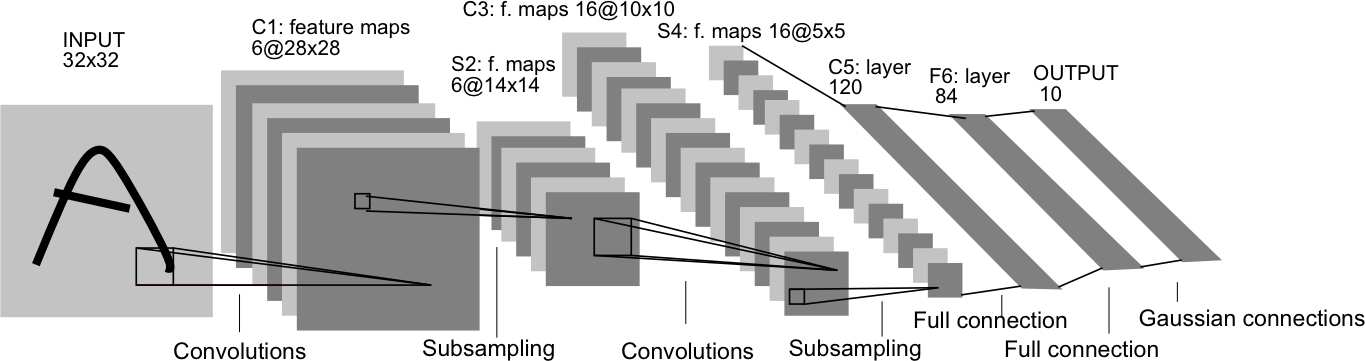
\includegraphics[width = 0.95 \textwidth]{chapters/images/lenet5.jpg}
    \caption[Architecture of LeNet-5]{Architecture of LeNet-5, Figure extracted from LeCun et al. 1998}
    \label{background:lenet5}
\end{figure}

LeNet was a big innovation for the time, since it obtains a $0.95 \%$ error rate on the MNIST dataset (corresponding to $99.05 \%$ accuracy), which is very close to human performance. Other kinds of classifiers such as K-Nearest-Neighbors with euclidean distance obtained $5 \%$ error rates, which shows the advantages of a CNNs.

LeNet set that initial standard for CNN design, starting with convolution and max-pooling blocks that are repeated a certain number of times, and perform feature extraction, followed by a couple of fully connected layers that perform classification or regression of those learned features. The network can be trained end-to-end using gradient descent.

A second milestone in CNNs is AlexNet \cite[-5em]{krizhevsky2012imagenet}, which is one of the first real deep neural networks trained on a large scale dataset. This network was designed to compete in the ImageNet Large Scale Visual Recognition Challenge \cite[-2em]{russakovsky2015imagenet}, where the task is to classify variable-sized images over 1000 different classes, with a training set containing 1.2 million images. It is a very difficult task due to the large training set, large number of classes, and many visual confusion between classes. \footnote[][2em]{For example, ImageNet contains many different races of dogs and cats, which a human cannot always visually distinguish.}

AlexNet unexpectedly won the ILSVRC competition in 2012, where most contenders were using classical computer vision methods and manually engineered features, but Kryzhevsky et al. showed that neural networks are competitive for this problem, and this is proven by the margin with the second place, of around $10 \%$ top-5 accuracy less than AlexNet.

The architecture of AlexNet is shown in Figure \ref{background:alexnet}, the network has 15 layers and approximately 60 million trainable parameters. AlexNet obtains $83.6$ \% top-5 accuracy on the ImageNet 2012 dataset, while the second place winner of the same competition obtains $73.8$ \% top-5 accuracy, showing the superior performance and capability of a deep neural network.

\begin{table}[t]
    \centering
    \begin{tabular}{@{}lll@{}}
        \hline
        Name					& Operation 							& Output Shape\\
        \hline
        Input					& Input image							& $(224, 224, 3)$ \\
        \hline
        Conv-1					& Conv($96$, $11 \times 11$, $S = 2$)	& $(55, 55, 96)$ \\
        MP-1					& Max-Pool($2 \times 2$)				& $(27, 27, 96)$ \\
        Conv-2					& Conv($256$, $5 \times 5$, $S = 1$)	& $(27, 27, 256)$ \\
        MP-2					& Max-Pool($2 \times 2$,)				& $(13, 13, 256)$ \\
        Conv-3					& Conv($384$, $3 \times 3$, $S = 1$)	& $(13, 13, 384)$ \\
        Conv-4					& Conv($384$, $3 \times 3$, $S = 1$)	& $(13, 13, 384)$ \\
        Conv-5					& Conv($256$, $3 \times 3$, $S = 1$)	& $(13, 13, 256)$ \\
        MP-3					& Max-Pool($2 \times 2$,)				& $(7, 7, 256)$ \\
        Flatten					& Flatten()								& $(7 \times 7 \times 256)$\\
        \hline
        FC-1					& FC($4096$, RELU)						& $(4096)$\\
        Dropout-1				& Dropout($0.5$)						& $(4096)$\\
        FC-2					& FC($4096$, ReLU)						& $(4096)$\\
        Dropout-2				& Dropout($0.5$)						& $(4096)$\\
        \hline
        FC-3					& FC($1000$, Softmax)					& $(1000)$\\
        \hline
    \end{tabular}
    \caption[Architecture of AlexNet as defined in Krizhevsky et al 2012]{Architecture of AlexNet as defined in Krizhevsky et al 2012. ReLU activations are used in each Convolutional Layer.}
    \label{background:alexnet}
\end{table}

Progress in the ImageNet competition has been constant over the years, producing advances in CNN architecture engineering. Pretty much all of the contenders after 2012 were using CNNs. In 2013 the VGG group at Oxford made a deeper version of AlexNet, which is typically just called VGG \cite{simonyan2014very}, with over 144 million parameters and obtaining $92 \%$ top-5 accuracy. The VGG networks use a simpler structure, with only $3 \times 3$ filters, and combining two consecutive convolutions both with $3 \times 3$ filters to simulate a bigger $5 \times 5$ filter.

In 2014 Google entered the competition with their GoogleNet \cite{szegedy2015going} architecture, which uses what they called the Inception module, that contains convolutions of multiple filter sizes combined with max pooling in a parallel structure, including $1 \times 1$ convolutions to learn features across channels/depth and $3 \times 3$ and $5 \times 5$ convolutions to learn spatial structure. GoogleNet obtains $93.3$ \% top-5 accuracy with 22 layers.

In 2015 Microsoft Research proposed Deep residual networks\cite{he2016deep}, which use a slightly different architecture that allows the network to be much more deep than possible before. A residual function is modeled as $F(x) + x$, where $x$ is the input to a set of layers, and $F(x)$ is the output of those layers. This addition operation is implemented as a skip connection that outputs the sum of the input and the output of a set of layers. The authors hypothesize that optimizing such structure is easier than the optimization process for a normal CNN, and they show this by building a much deeper (over 150) layer network that obtains $95.5$ \% top-5 accuracy.

\subsection{Discussion}

Different patterns in CNN architectures have emerged over the years, and overall there are some design choices that can be learned. In general a deeper network performs better, because it can learn higher level features which is only possible with a deep feature hierarchy. Seems that filters sizes do not have to be big (as in AlexNet), as most state of the art ImageNet CNNs use $3 \times 3$ and sometimes $5 \times 5$ filters. Even $1 \times 1$ filters are useful in order to influence information in the channels dimension.

A common pattern in the CNNs presented in this Section is that the number of filters increases with depth, and this makes sense, as deeper networks have smaller filter sizes and this has to be compensated by having more filters, which can represent a more rich feature hierarchy. There could be a one-to-one match between some features and specific filters, so in order to have more complex features, more filters are needed.

Overall, designing a neural network architecture for a specific task always requires a degree of experimentation. Designers should start with a small network, and expand it as needed, but only doing this kind of experimentation by evaluating on a evaluation set, and obtaining a final performance measure in a test set.

Neural network architectures can also be automatically designed by an algorithm. Popular choices are genetic algorithms \cite[-4em]{stanley2002evolving}, and newer techniques like Neural Architecture Search \cite[1em]{zoph2018learning} and Differentiable Architecture Search \cite[1em]{liu2018darts}.

In general automatic architecture design techniques have trouble achieving results that outperform the state of the art, as measured by classification performance in many common datasets (like ImageNet, CIFAR-10/100), only recent techniques are able to automatically produce an architecture that outperforms manually crafted architectures, so it can be expected that neural networks will be increasingly designed by algorithms and not by humans.

These kind of techniques are contributing to the long term goal of \textit{automatic machine learning}\cite[1em]{quanming2018taking}, where only labeled data is provided and the hyper-parameters of the architecture are automatically tuned in a validation subset, which has the potential of expanding the use of machine learning techniques to non-technical users.